\chapter{Integration}
\label{ch_hardware_integration}

\section{Software Integration}

Integration with third party software requires the compiled static or shared library and the two header files \textit{safecrypto.h} and \textit{safecrypto\_types.h}. When the build system is used to create and install \textit{libsafecrypto} these files will be present on the host system.

In order to verify that \textit{libsafecrypto} is correctly installed it is recommended that the first step of any integration task is to ensure that the correct library version number can be obtained from a simple test program such as that shown in \ref{fig:version_program}. When installed the header files will be found on the standard include path. When linking the compiler must link against the \textit{libsafecrypto} library, e.g. \textit{-lsafecrypto}.

\begin{figure}[H]
\centering
\begin{BVerbatim}
#include <stdlib.h>
#include <safecrypto.h>

int main(void)
{
    size_t i;
    UINT32 version;
    char *version_string;

    version = safecrypto_get_version();
    version_string = safecrypto_get_version_string();

    fprintf(stderr, "libsafecrypto v%08X (%s)\n",
        version, version_string);

    fprintf(stderr, "Supported schemes:\n");
    for (i=0; i<SC_SCHEME_MAX; i++) {
        fprintf(stderr, "%2lu: %s\n", i, sc_scheme_names[i]);
    }

    return EXIT_SUCCESS;
}
\end{BVerbatim}
\caption{Example version testing program}
\label{fig:version_program}
\end{figure}



\section{Hardware Integration}

This chapter discusses the method by which hardware implementations of Lattice-based cryptographic schemes will be integrated into the software library. This is intended to provide both a software interface for the hardware implementations and a means by which hardware acceleration of the software library can be achieved.

To this end the synchronisation of hardware and software will be achieved using worker threads to control, monitor and interact with any attached hardware device. Entire schemes or components of them can be offloaded in exactly the same manner as a multithreaded software implementation, allowing software functions and hardware implementations of those functions to be arbitrarily exchanged. This will improve the speed of development and testing of the codesigned software/hardware system.

\begin{figure}[h]
\centering
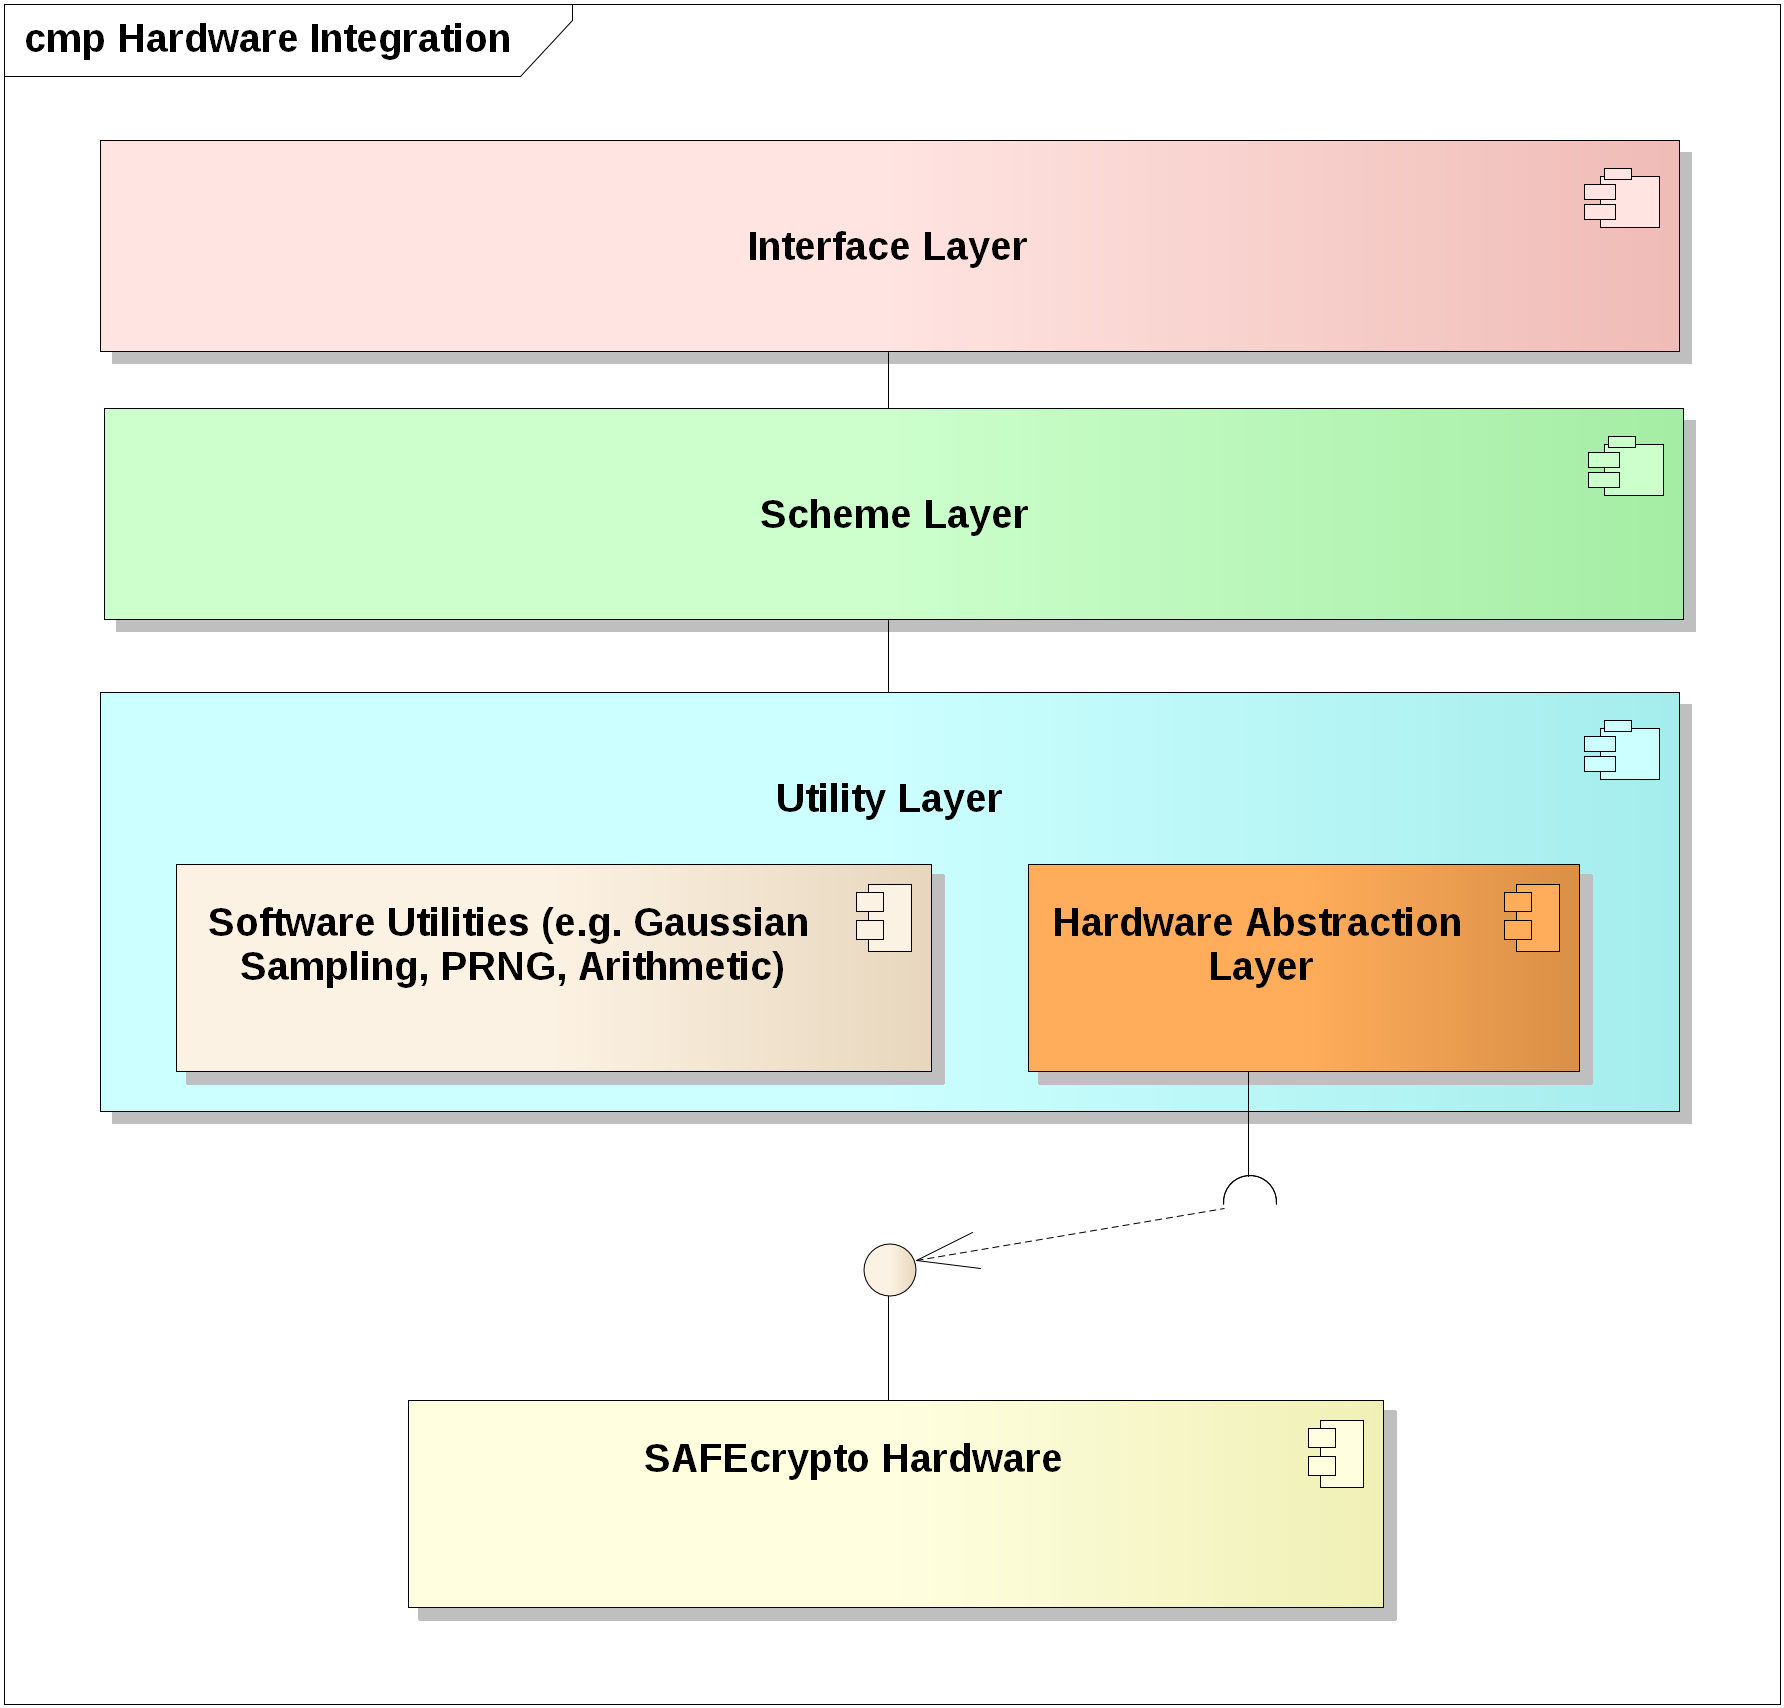
\includegraphics[width=0.7\textwidth]{hardware_integration.png}
\caption{Component diagram of a hardware only or hardware accelerated version of the \textit{SAFEcrypto} library}
\label{fig:safecrypto_hw_integration}
\end{figure}

To facilitate communication with any SAFEcrypto hardware a software component in the Utility Layer will provide a Hardware Abstraction Layer (HAL) (see Figure \ref{fig:safecrypto_hw_integration}). The HAL will abstract the interface to the hardware which will vary depending upon the hardware platform. The HAL will also provide a common API for any scheme to use SAFEcrypto hardware functionality.

For example, a Xilinx Zynq platform operates an Ubuntu Linux OS on its dual-core ARM A9 CPU while its FPGA provides a hardware resource that generates polynomials sampled from a specified Gaussian distribution. The HAL communicates with the hardware using memory-mapped registers and a dedicated interrupt line from the FPGA. A hardware-accelerated version of a Lattice-based cryptographic scheme can use a threadpool to queue tasks for the Gaussian Sampler hardware, where the tasks are dispatched to the hardware using the HAL. The status of the hardware is maintained by the HAL with the aid of the dedicated interrupt and a status register on the SAFEcrypto hardware. If the target platform is changed from an embedded ARM/Xilinx FPGA to an Intel Xeon-FPGA the SAFEcrypto software library must only change with respect to the implementation of the HAL.
